\documentclass{beamer}
\mode<presentation>
\usepackage{amsmath}
\usepackage{amssymb}
%\usepackage{advdate}
\usepackage{graphicx}
\usepackage{adjustbox}
\usepackage{subcaption}
\usepackage{enumitem}
\usepackage{multicol}
\usepackage{mathtools}
\usepackage{listings}
\usepackage{url}
\def\UrlBreaks{\do\/\do-}
\usetheme{Boadilla}
\usecolortheme{lily}
\setbeamertemplate{footline}
{
  \leavevmode%
  \hbox{%
  \begin{beamercolorbox}[wd=\paperwidth,ht=2.25ex,dp=1ex,right]{author in head/foot}%
    \insertframenumber{} / \inserttotalframenumber\hspace*{2ex} 
  \end{beamercolorbox}}%
  \vskip0pt%
}
\setbeamertemplate{navigation symbols}{}

\providecommand{\nCr}[2]{\,^{#1}C_{#2}} % nCr
\providecommand{\nPr}[2]{\,^{#1}P_{#2}} % nPr
\providecommand{\mbf}{\mathbf}
\providecommand{\pr}[1]{\ensuremath{\Pr\left(#1\right)}}
\providecommand{\qfunc}[1]{\ensuremath{Q\left(#1\right)}}
\providecommand{\sbrak}[1]{\ensuremath{{}\left[#1\right]}}
\providecommand{\lsbrak}[1]{\ensuremath{{}\left[#1\right.}}
\providecommand{\rsbrak}[1]{\ensuremath{{}\left.#1\right]}}
\providecommand{\brak}[1]{\ensuremath{\left(#1\right)}}
\providecommand{\lbrak}[1]{\ensuremath{\left(#1\right.}}
\providecommand{\rbrak}[1]{\ensuremath{\left.#1\right)}}
\providecommand{\cbrak}[1]{\ensuremath{\left\{#1\right\}}}
\providecommand{\lcbrak}[1]{\ensuremath{\left\{#1\right.}}
\providecommand{\rcbrak}[1]{\ensuremath{\left.#1\right\}}}
\theoremstyle{remark}
\newtheorem{rem}{Remark}
\newcommand{\sgn}{\mathop{\mathrm{sgn}}}
\providecommand{\abs}[1]{$\left\vert#1\right\vert$}
\providecommand{\res}[1]{\Res\displaylimits_{#1}} 
\providecommand{\norm}[1]{\lVert#1\rVert}
\providecommand{\mtx}[1]{\mathbf{#1}}
\providecommand{\mean}[1]{E$\left[ #1 \right]$}
\providecommand{\fourier}{\overset{\mathcal{F}}{ \rightleftharpoons}}
%\providecommand{\hilbert}{\overset{\mathcal{H}}{ \rightleftharpoons}}
\providecommand{\system}[1]{\overset{\mathcal{#1}}{ \longleftrightarrow}}
%\providecommand{\system}{\overset{\mathcal{H}}{ \longleftrightarrow}}
	%\newcommand{\solution}[2]{\textbf{Solution:}{#1}}
%\newcommand{\solution}{\noindent \textbf{Solution: }}
\providecommand{\dec}[2]{\ensuremath{\overset{#1}{\underset{#2}{\gtrless}}}}
\newcommand{\myvec}[1]{\ensuremath{\begin{pmatrix}#1\end{pmatrix}}}
\let\vec\mathbf

\lstset{
%language=C,
frame=single, 
breaklines=true,
columns=fullflexible
}

\numberwithin{equation}{section}

\title{4.13.93}
\author{AI25BTECH11024 - Pratyush Panda}
\begin{document}
\maketitle

\begin{frame}
\textbf{Question: } \\
Let $\Vec{P}$ be the image of the point $\brak{3,1,7}$ with respect to the plane $x-y+z=3$. Then the equation of the plane passing through $\Vec{P}$ and containing the straight line $\frac{x}{1}=\frac{y}{2}=\frac{z}{1}$ is
\begin{enumerate}
\item[a] $x+y-3z=0$
\item[b] $x-4y+7z=0$
\item[c] $x+3z=0$
\item[d] $2x-y=0$
\end{enumerate}
\end{frame}

\begin{frame}
\textbf{Solution: } \\
Let the vector $\Vec{A}=\myvec{3 \\ 1 \\ 7}$. \\

The given plane can be written as;
\begin{align}
\Vec{n_1}^T\Vec{X}=3 \hspace{1cm} where, \, \Vec{n_1}=\myvec{1 \\ -1 \\ 1}
\end{align}

And the line has the direction vector $\Vec{b}$=$\myvec{1 \\ 2 \\ 1}$

Now, the image of point $\Vec{A}$ with respect to the plane can be found out by the formula;
\begin{align}
\Vec{P}=\Vec{A}-\frac{2\brak{\Vec{n}^T\Vec{A}-3}}{||\Vec{n}||}\Vec{n}
\end{align}
\end{frame}

\begin{frame}
From putting the values in the formula, we get the point $\Vec{P}$ to be $\myvec{-1 \\ 5 \\ 3}$\\

Let the equation of the required plane be $\Vec{X}^T\Vec{n}=0$ since the plane contains the line and the line passes through the origin. \\

From the given constraints we can get the following equations;
\begin{align}
\Vec{P}^T\Vec{n}=0 && \Vec{b}^T\Vec{n}=0
\end{align}

If we combine the two equations we get;
\begin{align}
\myvec{P & b}^T\Vec{n}=\myvec{0 \\ 0}
\end{align}

On solving this equation we get $\Vec{n}=n.\myvec{1 \\ -4 \\ 7}$. The parameter can be taken as 1. \\
\end{frame}

\begin{frame}
Thus, the equation of the required plane is $\myvec{1 \\ -4 \\ 7}^T\Vec{X}=0$ or $x-4y+7z=0$.


\begin{figure}[H]
\centering
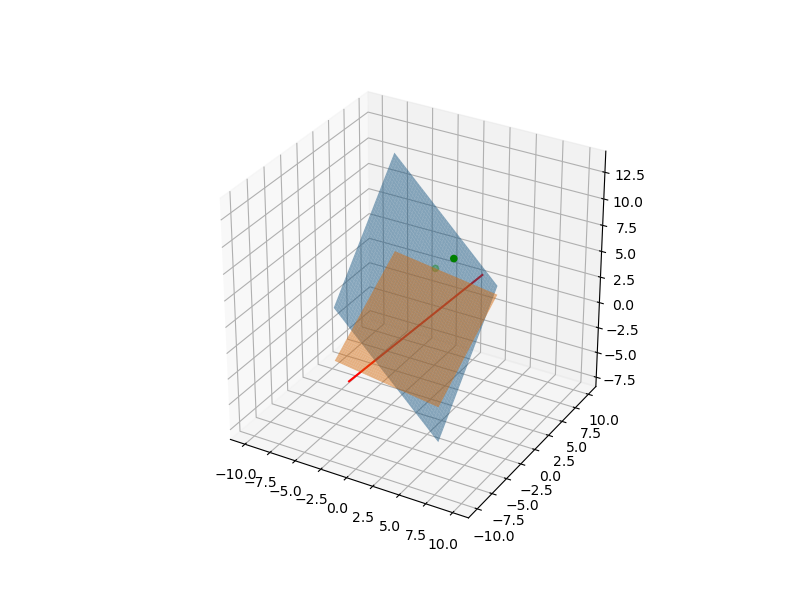
\includegraphics[width=0.7\columnwidth]{figs/img.png}
\caption*{}
\end{figure}
\end{frame}

\end{document}
